%
% Template LaTeX for 3 pages report of TI2P2
%
\documentclass[reprint, a4paper, nofootinbib, amsmath, amssymb, aps]{revtex4-1}
% 
%
\usepackage[english]{babel}
\usepackage[utf8]{inputenc}
%\usepackage{graphicx}
\usepackage{bm}
\usepackage[breaklinks]{hyperref}
\usepackage{amsmath}
\usepackage{mathrsfs}
\usepackage{amssymb}
\usepackage{float}
\usepackage{comment}
\usepackage{hyperref}
%\usepackage{mathtools}
% \newcommand*{\bfrac}[2]{\genfrac{}{}{0pt}{}{#1}{#2}}
%\usepackage{epstopdf}
\usepackage[pdftex]{graphicx,color}
%\epstopdfDeclareGraphicsRule{.pdf}{png}{.png}{convert #1 \OutputFile}
%\AppendGraphicsExtensions{.pdf}
% \usepackage{pdfpages} 
% \usepackage{lipsum}

\usepackage{caption}
\usepackage{tikz}
\usetikzlibrary{calc}
\usepackage{feynmf}
\usepackage{xcolor}
%\usepackage{etex}
\usepackage{textcomp}
\usepackage{marvosym}
\usepackage{wasysym}
\usepackage{amsthm}
\usepackage{comment}
\usepackage{qtree}
\usepackage{tikz-feynman}
\usepackage{array}
\usepackage[yyyymmdd]{datetime}
\begin{document}

\title{Cheat Sheet for new Ph.D student in the CMS team of IPHC}

\author{a Former Ph.D student}
\affiliation{Université de Strasbourg, IPHC, 23 rue du Loess 67037 Strasbourg, France}

\date{\today}

\maketitle

%%%%%%%%%%%%%%%%%%%
\section{Introduction}

First and foremost, welcome to the CMS team of Strasbourg and congratulation for being promoted to Ph.D student (or intern). This paper will try to quickly give you tools and useful links to better understand what are all the acronyms that you may encounter, LaTeX related things, CMS related things, etc (Nothing related to the Ecole Doctoral will be mentioned as rules given may change over years...). This list won't be exhaustive as there so many things to talk about but we hope that this will help you in any kind of way to fasten your progress in your work. For global IPHC commands, see: \href{https://twiki.cern.ch/twiki/bin/viewauth/CMS/IPHCusefulCommands#VScode}{IPHC useful commands}. There is also a nice VScode tutorial if you a not familiar with it. Good luck!  

\section{Acronyms}
    A set of Acronyms is defined in a Twiki page in : \href{https://twiki.cern.ch/twiki/bin/view/CMSPublic/WorkBookGlossary}{TwikiAcronyms}. Twiki pages are like wiki pages but for the CMS documentation of everything. By the time you read this, this may have changed to gitlab or something else.
%%%%%%%%%%%%%%%%%%%
\section{Compact Muon Solenoid detector }
    
    %----------------%
    \subsection{Point 5}

    The CMS detector is situated at one of the crossing point between the two beams of the LHC, also called Point 5 or P5. During your Ph.D, you will have to perform shift at P5 (trigger shifts, Data Quality Monitoring (DQM), Shift Leader, Data Acquisition System (DAQ), DCS Detector Control Status). There are different types of shifts, online (usually at P5) and offline (can be performed outside of P5 usually). A shift last 8 hours where you take care of one aspect of the detector mentioned above and have to communicate important information to others, the shift leader especially.
    It may change over time but a certain amount of shifts have to be performed by the CMS team of IPHC (there are quotas) and usually online shifts are the ones that are done to fulfill the quotas (even more points when doing night shifts). All the links related to the different shifts will not be given here as they may be updated quite often and are really specific. No worries, everything will be given to you by shifts coordinators when the time will come. \\
    Personal Experience: Trigger Shifts and DQM shifts are pretty cool and all kinds of shift help you better understand the experiment
    
    PS: Becareful, P5 is NOT on the Meyrin or the Prevessin sites. You need to take your car or the shuttle to get to P5 as CMS is wondering around in the countryside. There is also the car-sharing system of CMS. Taking the bike is not really recommended.
    


    \subsection{The detector}
    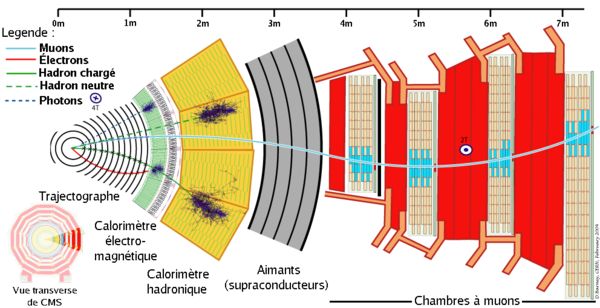
\includegraphics[height=4cm, width=8cm, trim= 0cm 0cm 0cm 0cm,clip]{Images/cmsAll.png}
    \label{fig: CMS}
    The CMS detector is 15 meter wide and 21 meter long. You can see a transverse view of CMS in Fig.\ref{fig: CMS}. The description will be a bit biased since the Strasbourg team is highly involved in the current tracker and its upgrade. At the very center, the closes part with respect to the interaction point is the beam pipe.Then comes the tracker that is divided into two parts (see Fig.\ref{fig: Tracker}) : Pixels and strips. Pixels are the innermost part of the tracker and also divided in to two parts: Barrel Pixels (BPIX) and Forward Pixels (FPIX). After the Pixels are the strips also divided into several parts: Tracker Inner Barrel (TIB), Tracker Outer Barrel (TOB). Then, there the two forward parts : the Tracker Inner Disks (TID) and Tracker End Caps (TEC). The characteristics (pitch, width, etc) of the modules of the silicon strip tracker change depending on where there are in the tracker.
    For the tracking, an iterative process is implemented to look for tracks. For electrons, it's slightly different due to Bremsstrahlung, the tracking is using the GaussianSum filter to take into account the information of photons. You may therefore encounter GSF electrons when coding :D. THe goal of the tracker is to reconstruct the tracks of charged particles (that deposits energy in the layers of the tracker)\\
    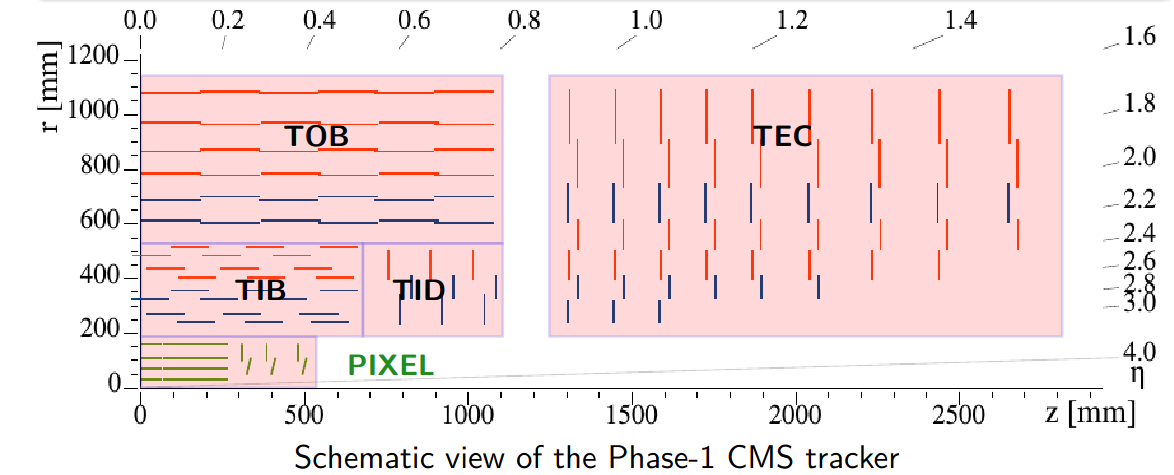
\includegraphics[height=4cm, width=8cm, trim= 0cm 0cm 0cm 0cm,clip]{Images/CMSTracker.png}\label{fig: Tracker}
    After the tracker comes the Electromagnetic and hadronic calorimeters. The former is used to detect energy deposits from photons and electrons (used for the GSF tracking). The hadronic calorimeter is used to detect energy deposits from both neutral and charged hadrons. \\
    Finally, there are the muons chambers. Again there are different types of subdetector for muon chambers like Resistive Plate Chambers (RPCs), Cathode Strip Chambers (CSC), Gas Electron Multiplier (GEM), Drift Tubes (DTs).Here is a small document to explain how each one of them works : \href{https://cds.cern.ch/record/2698492/files/Poster-2019-989.pdf}{Muon Poster} (click on Muon Poster).

    Since you are working in the Strasbourg team, some part of your work may be related to the tracker, here are a few links to better understand the tracker :
    \begin{itemize}
        \item \href{https://indico.cern.ch/event/1238081/timetable/#20230227}{Tracker training days 2023} : a lot of slides about everything concerning pixels and strips
        \item If you like reading more than going through slides, here is \href{https://cds.cern.ch/record/914891/files/jpconf6_41_011.pdf}{Doc Tracker}. Quite old but gives the basics
        \item Quantities related to the tracker : \href{http://cms.cern.ch/iCMS/jsp/openfile.jsp?type=DN&year=2020&files=DN2020_004.pdf}{Click}
    \end{itemize}
    
%%%%%%%%%%%%%%%%%%%
\section{LaTeX}
    You might need to use some LaTeX during your Ph.D, only examples will be given and a cheat sheet (all the examples are given as zip files that you can open in overleaf or you ;can just check the code):
    \begin{itemize}
        \item \href{https://wch.github.io/latexsheet/}{Cheat Sheet}
        \item FeynMan Diagrams : examples are given in the twiki page, see ppToXX 
        \item Poster : an exemple is given : Poster CMS Week ...
        \item Of course, there are many more things to know but this will give you the basics if you are a beginner
    \end{itemize}

    You will see that the TikZ library is used and is kinda common to draw shapes, add things to already existing plots, Feynman diagrams, etc. When using the tikzFeynman library or tikz in general, you may need to change the compiler of overleaf to lualatex in the Menu on the top left.
    
\section{root}

 Only few things will be given as there are not much things to know  about ROOT.
 Be always careful about the version of root you are using as you may face root version incompatibility. You can change the version of root you are using by doing this command  on the uiX: \\
 \begin{center}
     $\rightarrow$ ls  /libcern/root (to check which version are available) \\
     $\rightarrow$ source /libcern/root/6.24.06/centos7.6-x86\_64/bin/thisroot.sh to change of version (for example)
 \end{center}

    From a root Ntuple where you have stored branches, you can open the file in a TBrowser and do :
    \begin{center}
        "name of the tree"-$>$MakeClass("toto")
    \end{center}
  It will create a .c and .h file that you can use directly to run over the events of the ntuple.\\
  Again, with a Ntuple, you can use the edmDumpEventContent $<$name of file$>$ to check the collections available in the file
  
  
\section{Physics Analysis}
Madgraph / generation, pythia8, powheg

Gen-Sim, Raw, reco, AOD, MniAOD, Nanoaod
    We have discussed dataformat  in a section above. CERN is actually pushing towards NanoAOD but RECO, AOD and MiniAOD can be used. For your analysis, there is a high chance that you work with at least AOD if MiniAOD if not nanoAOD :D. \\
    Depending on the data format that you are using, the collection of tracks (codewise) that you can use is different. 
https://twiki.cern.ch/twiki/bin/view/CMSPublic/WorkBookAnalysisOverviewIntroduction
    https://twiki.cern.ch/twiki/bin/view/CMSPublic/WorkBook
    
\subsection{Analysis Strategy}
\subsection{Run 2}
    Global information about Run 2 : \\
    \href{https://twiki.cern.ch/twiki/bin/view/CMS/PdmVRun2LegacyAnalysis}{Global Information} \\
    \href{https://twiki.cern.ch/twiki/bin/viewauth/CMS/PdmVAnalysisSummaryTable}{Summary of what to use} \\
    Then, the MC simulation may not represent the data because data is hard to reproduce correctly. There can be detector effect to be taken into account. All these things need corrections that can be found in the following links : 
    \href{https://twiki.cern.ch/twiki/bin/view/CMS/PileupJetIDUL#Recommendations_for_2018_UL_data}{PileUp reweighting info} \\
    \href{https://twiki.cern.ch/twiki/bin/view/CMS/LumiRecommendationsRun2}{LumiREcommendations} \\
    \href{https://twiki.cern.ch/twiki/bin/view/CMSPublic/WorkBookJetEnergyResolution}{Jet Energy resolution} \\
    \href{https://indico.cern.ch/event/1247210/sessions/478562/attachments/2587866/4465075/MuonPOG_tutorial_part2.pdf}{MuonSF} \\
    \href{https://twiki.cern.ch/twiki/bin/viewauth/CMS/SWGuideMuonIdRun2}{MuonID} \\
    \href{https://twiki.cern.ch/twiki/bin/view/CMS/RochcorMuon}{RochesterCorrections}\\
    There are many more things to know but this give you a firstview of what to check. You can also check the page to also summarizes kind of everything : \href{https://twiki.cern.ch/twiki/bin/view/CMS/TopSystematics}{TopSyst} 
    
\subsection{Run 3}
    Global information about Run 3 : \href{https://twiki.cern.ch/twiki/bin/view/CMS/PdmVRun3Analysis#Run_3_Analysis}{Click}

    You can follow the links for Run 2, there may redirect you to Run 3 pages :D or still be valid for Run 3.
\subsection{Physics Object}
    It may be useful when you are starting an analysis from scratch. If you are using an already existing framework for your analysis, then you might nit care about the following. \\
    For the different data format, you do not manipulate the physics object in the same way, so here are two workbooks for the MiniAOD and NanoAOD : \\
    \href{https://twiki.cern.ch/twiki/bin/view/CMSPublic/WorkBookMiniAOD2017}{MiniAOD}\\
    \href{https://twiki.cern.ch/twiki/bin/view/CMSPublic/WorkBookNanoAOD}{NanoAOD}\\
    Yeah, we know it is from Run 2, welcome to CMS where nothing is really up-to-date.



\subsection{Combine}


    Once you have implemented your analysis strategy, you meed to set limits on some cross-sections, couplings, masses, or even define scale factors. A tool has been developed within the CMS collaboration and made available to anyone : \href{https://cms-analysis.github.io/HiggsAnalysis-CombinedLimit/latest/}{Combine}. It was first used to discover the Higgs boson back in 2012. Now, it  has a general purpose and really powerful. However, it takes quite some time to fully grasp and understand everything. Following the tutorial first is the best (and a decent understanding of statistics is needed)- \href{https://cms-analysis.github.io/HiggsAnalysis-CombinedLimit/latest/part5/longexercise/}{Tutorial}. You will probably see some Brazilian plots in your time here, and they may come from Combine.

\section{crab}
\href{https://twiki.cern.ch/twiki/bin/view/CMSPublic/CRAB3ConfigurationFile}{CrabconfigFile}
 During your Ph.D, you may need to run on MC simulation samples with millions of events. You can do that on your local computer but you may finish your Ph.D  before you finish analyzing the events. To address this issue, you have access to a grid. For that, you need a certificate that needs to be updated once every year. \href{https://twiki.cern.ch/twiki/bin/view/CMSPublic/WorkBookChapter5}{CMSCertificate} and \href{https://indico.in2p3.fr/event/32895/}{Yannick's slides}. Once you have your certificate, you can submit crab jobs using the following commands (in a cms envrionnement area): 
 
'source /cvmfs/cms.cern.ch/crab3/crab.sh' \\
'voms-proxy-init -rfc -voms cms -valid 192:00'\\
'crab submit -c crab\_config\_mc\_2018.py' \\

where crab\_config\_mc\_2018.py is a configuration file for your crab jobs. A version of config file is given in the git repository (multicrab) that allows to launch on multiple  MC sample.

You have to use slightly different commands for that :
./multicrab --crabCmd submit (to launch the jobs)

./multicrab --crabCmd status --workArea ./$<$work\_directory$>$ (to get the status of the jobs : failed, idle , running ,finished or not submitted)\\
./multicrab --crabCmd kill --workArea ./$<$work\_directory$>$ (to kill the jobs )\\
./multicrab --crabCmd resubmit --workArea ./$<$work\_directory$>$ (resubmit failed jobs)\\

To get the outpule files, you need to use the gfal commands :
(You have to do that without setting the cmsenv but only :\\
source /cvmfs/cms.cern.ch/crab3/crab.sh )\\
gfal-ls davs://sbgdcache.in2p3.fr/cms/phedex/store/user/$<$Your directory$>$\\
gfal-copy -r davs://sbgdcache.in2p3.fr/cms/phedex/store/user/$<$Your directory$>$ \\
Then you will probably need to hadd (gather together) the different output files and you are done.

%%%%%%%%%%%%%%%%%%%
\section{Conclusion}

I hope that it somehow helped you. It is not exhaustive and probably not up-to-date when you will be reading it but it gives hints or potential solution to your issues. Good luck in your Ph.D (or internship)\\

La Relève 
%%%%%%%%%%%%%%%%%%%%%%%%%%%%%%

\end{document}
